\subsection{可制御性}

状態フィードバックで極を動かす前に、そもそも入力が状態空間のどの方向へ作用できるかを調べる必要がある。ここでは有限次元の連続時間線形時不変系
\begin{equation}
  \dot{x}=Ax+Bu,\qquad x\in\R^n,\quad u\in\R^m
\end{equation}
を考える。入力 $u(t)$ は区分的連続で、振幅制限や速度制限はまだ入れない。したがって可制御性は、アクチュエータが理想的に使えるという代数的な判定であり、入力飽和を含む実装可能性とは別の概念である。

\begin{definition}[可到達性と可制御性]
ある時刻 $T>0$ が存在して、任意の初期状態 $x(0)=x_0$ から任意の終端状態 $x(T)=x_f$ へ入力で移せるとき、対 $(A,B)$ は可制御であるという。特に $x_0=0$ から到達できる状態の集合を可到達部分空間という。連続時間の有限次元線形時不変系では、この可到達性と可制御性は同じランク条件で判定できる。
\end{definition}

入力が作る状態変化は、解公式
\begin{equation}
  x(T)-e^{AT}x_0
  =\int_0^T e^{A(T-\tau)}Bu(\tau)\,\dd\tau
  \label{eq:reachable-increment}
\end{equation}
で表される。右辺に現れる $e^{A(T-\tau)}B$ は、入力行列 $B$ の列ベクトルを自然運動 $A$ で回し、混ぜ、伸縮させた方向である。したがって「入力が直接押せる方向」だけでなく、「対象自身の結合を通って入力が広がる方向」も数えなければならない。

\begin{theorem}[Kalman の可制御性ランク条件]
連続時間線形時不変系 $(A,B)$ が可制御であるための必要十分条件は
\begin{equation}
  \rank\mathcal{C}=n,\qquad
  \mathcal{C}=\begin{bmatrix}B&AB&A^2B&\cdots&A^{n-1}B\end{bmatrix}
  \label{eq:kalman-controllability-matrix}
\end{equation}
である。この $\mathcal{C}$ を可制御行列という。
\end{theorem}

\begin{derivation}
まず、行列指数関数の級数表示より
\begin{equation}
  e^{A\sigma}B
  =\left(I+A\sigma+\frac{A^2\sigma^2}{2!}+\cdots\right)B
\end{equation}
である。Cayley--Hamilton の定理により $A^n,A^{n+1},\ldots$ は $I,A,\ldots,A^{n-1}$ の線形結合で表せるので、任意の $\sigma$ に対して $e^{A\sigma}B$ の列空間は $\mathcal{C}$ の列空間に含まれる。したがって \weq{reachable-increment} で作れる状態変化は、すべて
\begin{equation}
  \operatorname{Im}\mathcal{C}
  =\operatorname{span}\{B,AB,\ldots,A^{n-1}B\}
\end{equation}
に入る。もし $\rank\mathcal{C}<n$ なら、この部分空間に直交する非零ベクトル $q$ が存在し、$q^\T A^iB=0$ が $i=0,\ldots,n-1$ で成り立つため、その方向の成分は入力で作れない。

逆に $\rank\mathcal{C}=n$ とする。有限時間 $T>0$ に対し、可制御 Gramian を
\begin{equation}
  W_c(T)=\int_0^T e^{A(T-\tau)}BB^\T e^{A^\T(T-\tau)}\,\dd\tau
\end{equation}
とおく。任意の非零 $q$ について
\begin{equation}
  q^\T W_c(T)q
  =\int_0^T \norm{B^\T e^{A^\T(T-\tau)}q}^2\,\dd\tau
\end{equation}
である。この値が 0 なら $B^\T e^{A^\T s}q=0$ がすべての $s$ で成り立つ。$s=0$ における微分を順に見ると $B^\T(A^\T)^iq=0$、すなわち $q^\T A^iB=0$ が $i=0,\ldots,n-1$ で成り立つが、これは $\rank\mathcal{C}=n$ と矛盾する。したがって $W_c(T)$ は正定値であり、逆行列を持つ。

任意の終端偏差
\begin{equation}
  z=x_f-e^{AT}x_0
\end{equation}
に対して
\begin{equation}
  u(\tau)=B^\T e^{A^\T(T-\tau)}W_c(T)^{-1}z
\end{equation}
と選べば、\weq{reachable-increment} の右辺は
\begin{equation}
  W_c(T)W_c(T)^{-1}z=z
\end{equation}
となる。よって任意の $x_0$ から任意の $x_f$ へ移せる。
\end{derivation}

可制御行列は、倒立振子のように入力が直接すべての状態へ入らない系で重要になる。台車へ加える力はまず台車速度に作用し、力学的な結合を通じて振子角へ伝わる。この「何回 $A$ を通ると別の状態方向へ届くか」を、$B,AB,A^2B,\ldots$ が数えている。

二状態の例では、$B$ は入力が瞬時に押す方向であり、$AB$ はその変化が対象の内部結合を一回通った後に現れる方向である。これらが平面上で同一直線に重なるなら、入力で作れる状態変化は一次元に閉じる。可観測性でも同様に、$C^\T$ は出力がその瞬間に測っている方向、$A^\T C^\T$ は出力微分に現れる方向を表す。図\ref{fig:controllability-observability-examples} は、この対応を正規化した状態平面上で比較したものである。図の矢印は方向だけを表し、実際の状態量の単位やスケールは各モデルの状態定義に依存する。

\begin{figure}[tb]
\centering
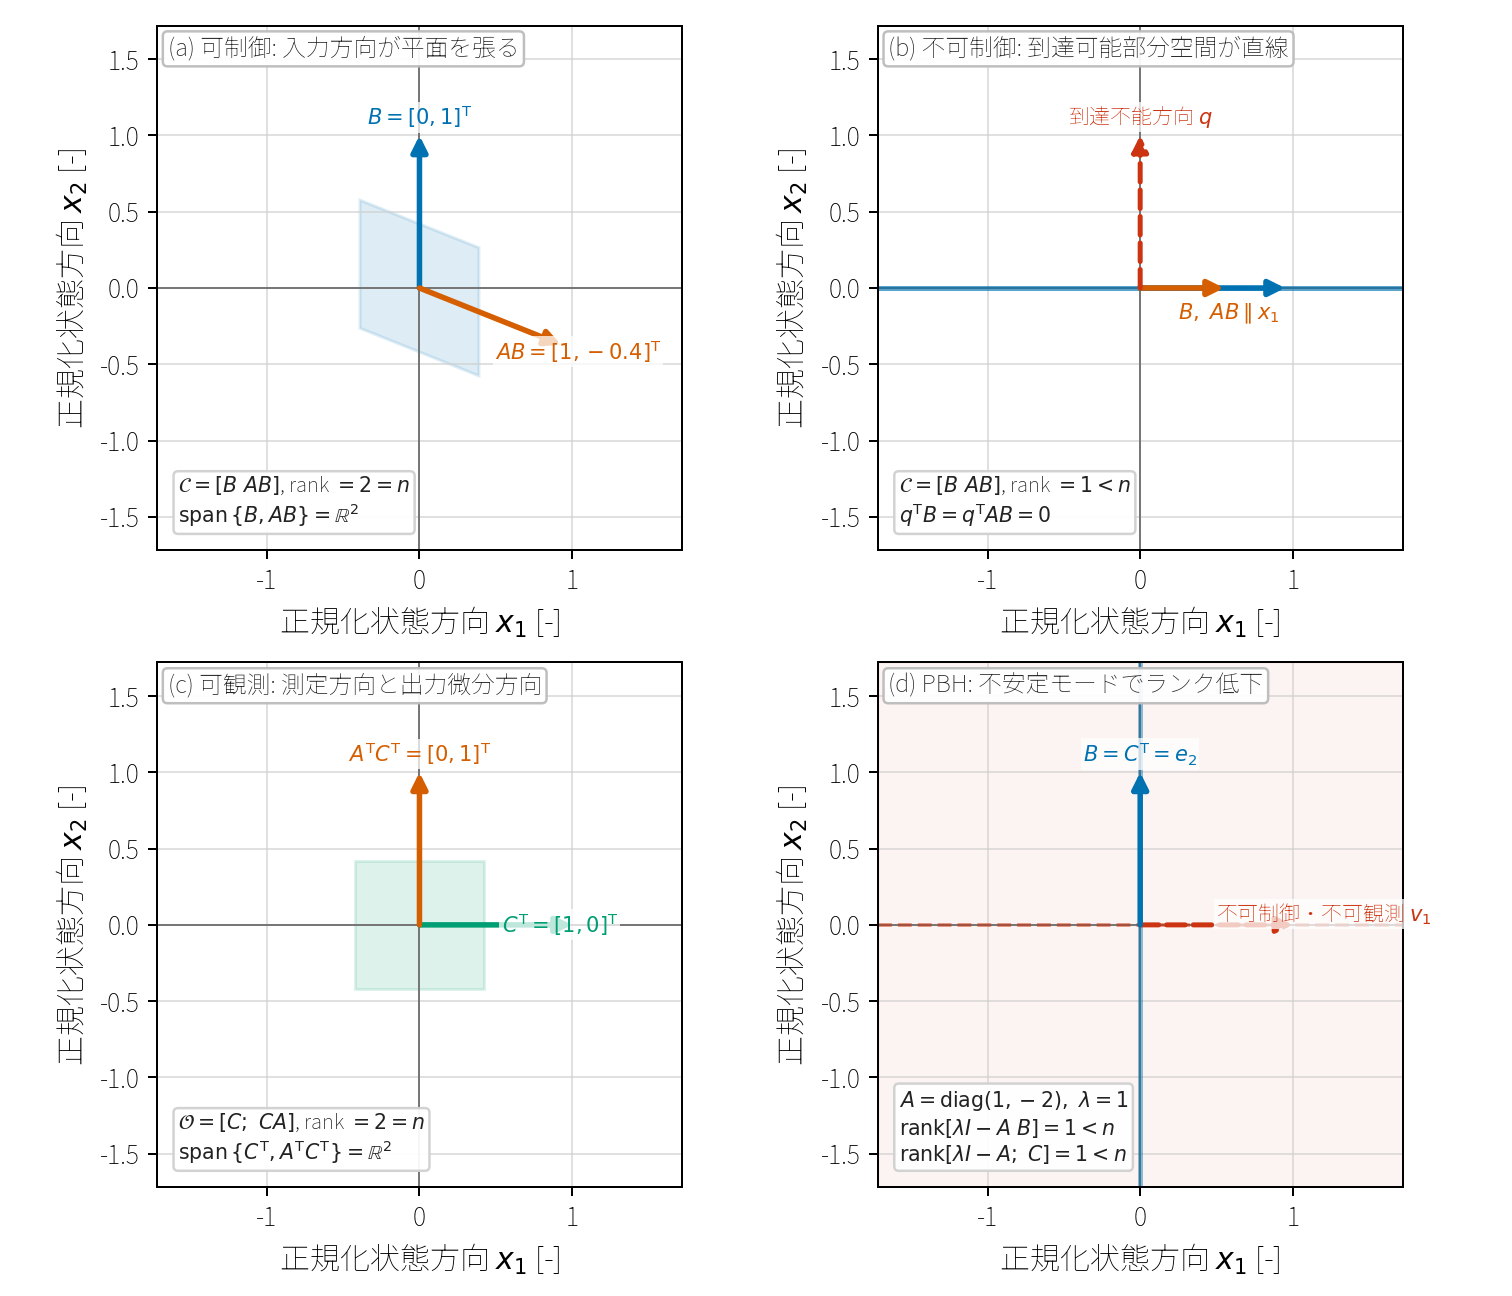
\includegraphics[width=0.96\linewidth,bb=0 0 1512 1296]{figures/controllability_observability_examples.png}
\caption{可制御性、可観測性、PBH 条件の幾何的な比較。左上は $A=\left[\begin{smallmatrix}0&1\\-2&-0.4\end{smallmatrix}\right]$、$B=\left[\begin{smallmatrix}0\\1\end{smallmatrix}\right]$ としたとき、$B$ と $AB$ が二次元平面を張り $\rank\mathcal{C}=2$ となる例を示す。右上は $B$ と $AB$ が同一直線上に残り、$x_2$ 方向が到達不能になるため $\rank\mathcal{C}=1$ へ落ちる例である。左下は $C=\left[\begin{smallmatrix}1&0\end{smallmatrix}\right]$ としたとき、$C^\T$ と $A^\T C^\T$ が二次元平面を張り $\rank\mathcal{O}=2$ となる例を示す。右下は $A=\operatorname{diag}(1,-2)$、$B=C^\T=e_2$ としたとき、不安定固有方向 $e_1$ が入力方向にも測定方向にも含まれず、$\lambda=1$ の PBH 行列ランクが $1<2$ へ低下する例である。}
\label{fig:controllability-observability-examples}
\end{figure}

図\ref{fig:controllability-observability-examples} の各パネルは、矢印の幾何とランク計算が同じ判定を与えることを数値で示している。左上では
\begin{equation}
  A=\begin{bmatrix}0&1\\-2&-0.4\end{bmatrix},\qquad
  B=\begin{bmatrix}0\\1\end{bmatrix},\qquad
  AB=\begin{bmatrix}1\\-0.4\end{bmatrix}
\end{equation}
なので、
\begin{equation}
  \mathcal{C}=\begin{bmatrix}B&AB\end{bmatrix}
  =\begin{bmatrix}0&1\\1&-0.4\end{bmatrix},\qquad
  \rank\mathcal{C}=2
\end{equation}
である。二つの列は同一直線上になく、入力方向と一回内部結合を通った方向が平面全体を張る。右上では
\begin{equation}
  A=\begin{bmatrix}0.55&0\\0&-0.2\end{bmatrix},\qquad
  B=\begin{bmatrix}1\\0\end{bmatrix},\qquad
  AB=\begin{bmatrix}0.55\\0\end{bmatrix}
\end{equation}
となり、
\begin{equation}
  \mathcal{C}
  =\begin{bmatrix}1&0.55\\0&0\end{bmatrix},\qquad
  \rank\mathcal{C}=1
\end{equation}
である。到達可能部分空間は $x_1$ 軸だけに閉じ、$q=e_2$ 方向の成分は $q^\T B=q^\T AB=0$ のまま入力から外れる。

左下の可観測な例では同じ $A$ に対して $C=\begin{bmatrix}1&0\end{bmatrix}$ とおくため、
\begin{equation}
  CA=\begin{bmatrix}0&1\end{bmatrix},\qquad
  \mathcal{O}=\begin{bmatrix}C\\CA\end{bmatrix}
  =\begin{bmatrix}1&0\\0&1\end{bmatrix},\qquad
  \rank\mathcal{O}=2
\end{equation}
である。測定が直接見る方向 $C^\T$ と、出力微分に現れる方向 $A^\T C^\T$ が直交する二方向を作るので、初期状態の二成分を出力履歴から分けられる。

右下では
\begin{equation}
  A=\operatorname{diag}(1,-2),\qquad
  B=C^\T=e_2,\qquad C=\begin{bmatrix}0&1\end{bmatrix}
\end{equation}
であり、不安定固有方向は $e_1$、入力と測定が向く方向は安定固有方向 $e_2$ である。$\lambda=1$ では
\begin{equation}
  \begin{bmatrix}\lambda I-A&B\end{bmatrix}_{\lambda=1}
  =
  \begin{bmatrix}0&0&0\\0&3&1\end{bmatrix},\qquad
  \begin{bmatrix}\lambda I-A\\C\end{bmatrix}_{\lambda=1}
  =
  \begin{bmatrix}0&0\\0&3\\0&1\end{bmatrix}
\end{equation}
となり、どちらの PBH 行列もランクは $1<2$ である。一方、$\lambda=-2$ では
\begin{equation}
  \begin{bmatrix}\lambda I-A&B\end{bmatrix}_{\lambda=-2}
  =
  \begin{bmatrix}-3&0&0\\0&0&1\end{bmatrix},\qquad
  \begin{bmatrix}\lambda I-A\\C\end{bmatrix}_{\lambda=-2}
  =
  \begin{bmatrix}-3&0\\0&0\\0&1\end{bmatrix}
\end{equation}
となり、どちらもランクは $2$ である。したがって問題は安定な $-2$ モードではなく、不安定な $\lambda=1$ モードが入力にも出力にも現れない点にある。$e_1$ 方向では $q^\T B=0$ なので状態フィードバックを入れてもその極を左半平面へ移せず、$Ce_1=0$ なのでオブザーバ補正を入れてもその推定誤差モードを減衰させられない。この不安定な隠れ方向が、安定化可能性と検出可能性を同時に失わせる。

\subsubsection{PBH 可制御性判別}

Kalman のランク条件は全方向をまとめて調べる。一方、どの固有モードが入力から見えていないかを知りたいときは、Popov--Belevitch--Hautus の判別法、通常 PBH 判別法を使う。

\begin{theorem}[PBH 可制御性判別]
対 $(A,B)$ が可制御であるための必要十分条件は、$A$ のすべての固有値 $\lambda\in\mathbb{C}$ について
\begin{equation}
  \rank\begin{bmatrix}\lambda I-A&B\end{bmatrix}=n
  \label{eq:pbh-controllability}
\end{equation}
が成り立つことである。これは、$q^\ast A=\lambda q^\ast$ を満たす非零の左固有ベクトル $q$ で
\begin{equation}
  q^\ast B=0
\end{equation}
となるものが存在しない、という条件と同値である。
\end{theorem}

PBH 判別法に固有ベクトル方向が現れる理由は、状態を固有モードの重ね合わせとして分解すると明確になる。左固有ベクトル $q$ によるモード座標 $\eta=q^\ast x$ をとると
\begin{equation}
  \dot{\eta}=q^\ast\dot{x}=q^\ast Ax+q^\ast Bu
  =\lambda q^\ast x+q^\ast Bu
  =\lambda\eta+q^\ast Bu
\end{equation}
である。もし $q^\ast B=0$ なら、このモード座標は
\begin{equation}
  \dot{\eta}=\lambda\eta
\end{equation}
となり、入力をどのように選んでも直接変えられない。したがって、単に固有値が安定か不安定かを見るだけでなく、その固有値に対応する方向へ入力が射影されているかを調べる必要がある。同じ固有値をもつ方向が複数ある場合、一部の方向だけが可制御で、別の方向が入力から外れていることもある。

可制御でないモードが存在しても、そのモードがすべて安定なら、閉ループ全体を安定にできる場合がある。この性質を安定化可能性という。可制御性はすべての極を任意に置くための条件であり、安定化可能性は少なくとも不安定なモードを制御できるための条件である。この違いは、PBH 判別法を不安定モードだけに制限した条件として定式化できる。

\subsection{可観測性}

状態を測れるか、または出力から推定できるかは可観測性で決まる。既知入力 $u$ と直達項 $D$ がある場合、$Du$ は出力から差し引けるので、初期状態の識別だけを考えると
\begin{equation}
  y_0(t)=Ce^{At}x(0)
\end{equation}
を調べればよい。可観測性は、異なる初期状態が異なる出力履歴を作るかという性質である。

\begin{definition}[可観測性]
ある有限時間区間 $0\le t\le T$ の出力履歴と既知入力から初期状態 $x(0)$ を一意に決められるとき、対 $(A,C)$ は可観測であるという。
\end{definition}

\begin{theorem}[Kalman の可観測性ランク条件]
連続時間線形時不変系 $(A,C)$ が可観測であるための必要十分条件は
\begin{equation}
  \rank\mathcal{O}=n,\qquad
  \mathcal{O}=\begin{bmatrix}C\\ CA\\ CA^2\\ \vdots\\ CA^{n-1}\end{bmatrix}
  \label{eq:kalman-observability-matrix}
\end{equation}
である。この $\mathcal{O}$ を可観測行列という。
\end{theorem}

\begin{derivation}
二つの初期状態 $x_a(0)$ と $x_b(0)$ が同じ出力を作るとする。その差を $\xi=x_a(0)-x_b(0)$ とおけば、出力差は
\begin{equation}
  \Delta y(t)=Ce^{At}\xi
\end{equation}
である。これがすべての $t$ で 0 なら、$t=0$ における値と微分から
\begin{equation}
  C\xi=0,\quad CA\xi=0,\quad CA^2\xi=0,\quad \ldots
\end{equation}
が得られる。Cayley--Hamilton の定理により $A^n$ 以上の冪は $I,A,\ldots,A^{n-1}$ の線形結合で表せるので、必要なのは
\begin{equation}
  \mathcal{O}\xi=0
\end{equation}
だけである。$\rank\mathcal{O}=n$ なら零空間は $\xi=0$ だけなので、同じ出力履歴を作る異なる初期状態は存在しない。逆に $\rank\mathcal{O}<n$ なら非零の $\xi$ で $\mathcal{O}\xi=0$ となるものがあり、その状態差は出力に現れない。
\end{derivation}

可制御性と可観測性は双対である。$(A,B)$ の可制御性は $(A^\T,B^\T)$ の可観測性と同じ形で判定できる。また、$(A,C)$ の可観測性は $(A^\T,C^\T)$ の可制御性と同じ形で判定できる。この双対性により、状態フィードバックの極配置とオブザーバゲインの極配置は、行列を転置した同じ代数問題として扱える。

\subsubsection{PBH 可観測性判別}

\begin{theorem}[PBH 可観測性判別]
対 $(A,C)$ が可観測であるための必要十分条件は、$A$ のすべての固有値 $\lambda\in\mathbb{C}$ について
\begin{equation}
  \rank\begin{bmatrix}\lambda I-A\\ C\end{bmatrix}=n
  \label{eq:pbh-observability}
\end{equation}
が成り立つことである。これは、$Av=\lambda v$ を満たす非零の右固有ベクトル $v$ で
\begin{equation}
  Cv=0
\end{equation}
となるものが存在しない、という条件と同値である。
\end{theorem}

右固有ベクトル $v$ 方向の初期状態 $x(0)=v$ は、入力を取り除いて見ると
\begin{equation}
  x(t)=e^{\lambda t}v,\qquad
  y(t)=Ce^{\lambda t}v=e^{\lambda t}Cv
\end{equation}
という出力を作る。もし $Cv=0$ なら、その固有モードはどれだけ成長または振動しても出力には現れない。これが PBH 可観測性判別で固有ベクトル方向を見る理由である。固有値の数値だけを見ても、センサがそのモードの方向を見ているかどうかは分からない。

可観測でないモードがあっても、そのモードがすべて安定なら、推定誤差の安定性には十分な場合がある。この性質を検出可能性という。検出可能性は、出力に現れない不安定モードがないことを求める条件であり、カルマンフィルタや LQG で重要になる。可観測性が全状態の復元を要求するのに対し、検出可能性は不安定な未検出成分を残さないことを要求する。

\subsubsection{安定化可能性と検出可能性の PBH 条件}

ここでは連続時間の有限次元線形時不変系を対象とし、$\sigma(A)$ を $A$ の固有値集合とする。行列 $A$ が Hurwitz であるとは、すべての $\lambda\in\sigma(A)$ が $\Re\lambda<0$ を満たすことをいう。したがって安定化設計で問題になるモードは、$\Re\lambda\ge0$ を満たす不安定または非減衰のモードである。離散時間系では、Hurwitz 安定を Schur 安定に、条件 $\Re\lambda\ge0$ を $|\lambda|\ge1$ に置き換える。

\begin{definition}[安定化可能性と検出可能性]
対 $(A,B)$ が安定化可能であるとは、ある行列 $K\in\R^{m\times n}$ が存在して $A-BK$ が Hurwitz になることをいう。対 $(A,C)$ が検出可能であるとは、ある行列 $L\in\R^{n\times p}$ が存在して $A-LC$ が Hurwitz になることをいう。
\end{definition}

\begin{theorem}[PBH--Hautus の安定化可能性判別]
対 $(A,B)$ が安定化可能であるための必要十分条件は、$A$ のすべての固有値 $\lambda\in\sigma(A)$ のうち $\Re\lambda\ge0$ を満たすものについて
\begin{equation}
  \rank\begin{bmatrix}\lambda I-A&B\end{bmatrix}=n
  \label{eq:pbh-stabilizability}
\end{equation}
が成り立つことである。等価に、$q^\ast A=\lambda q^\ast$ かつ $q^\ast B=0$ を満たす非零の左固有ベクトル $q$ が存在するなら、その固有値は必ず $\Re\lambda<0$ でなければならない。
\end{theorem}

\begin{theorem}[PBH--Hautus の検出可能性判別]
対 $(A,C)$ が検出可能であるための必要十分条件は、$A$ のすべての固有値 $\lambda\in\sigma(A)$ のうち $\Re\lambda\ge0$ を満たすものについて
\begin{equation}
  \rank\begin{bmatrix}\lambda I-A\\ C\end{bmatrix}=n
  \label{eq:pbh-detectability}
\end{equation}
が成り立つことである。等価に、$Av=\lambda v$ かつ $Cv=0$ を満たす非零の右固有ベクトル $v$ が存在するなら、その固有値は必ず $\Re\lambda<0$ でなければならない。
\end{theorem}

これらの条件は、完全な可制御性と可観測性が十分条件ではあるが必要条件ではないことを示している。可制御性の PBH 判別はすべての固有値について \weq{pbh-controllability} を要求するため、安定な不可制御モードも許さない。これに対し、安定化可能性では安定な不可制御モードを残してよい。状態フィードバックでその極を任意に動かすことはできないが、もともと減衰するため閉ループの漸近安定性を破壊しない。同様に、可観測性はすべての初期状態を出力履歴から一意に復元する条件であるが、検出可能性では安定な不可観測モードを許す。オブザーバはその成分を出力補正で直接同定できないが、推定誤差が自然に減衰するなら $A-LC$ を Hurwitz にできる。

対角化されたモードでこの差を確認する。状態 $x=\begin{bmatrix}x_1&x_2\end{bmatrix}^\T$ に対し
\begin{equation}
  A=\begin{bmatrix}1&0\\0&-2\end{bmatrix},\qquad
  B=\begin{bmatrix}1\\0\end{bmatrix},\qquad
  C=\begin{bmatrix}1&0\end{bmatrix}
  \label{eq:modal-stabilizable-detectable-example}
\end{equation}
を考える。$x_1$ は固有値 $1$ の不安定モード、$x_2$ は固有値 $-2$ の安定モードである。可制御行列と可観測行列は
\begin{equation}
  \mathcal{C}=\begin{bmatrix}B&AB\end{bmatrix}
  =\begin{bmatrix}1&1\\0&0\end{bmatrix},\qquad
  \mathcal{O}=\begin{bmatrix}C\\CA\end{bmatrix}
  =\begin{bmatrix}1&0\\1&0\end{bmatrix}
\end{equation}
なので、どちらもランクは $1$ であり、完全には可制御でも可観測でもない。しかし不安定な固有値 $\lambda=1$ に限れば
\begin{equation}
  \begin{bmatrix}\lambda I-A&B\end{bmatrix}_{\lambda=1}
  =
  \begin{bmatrix}0&0&1\\0&3&0\end{bmatrix},\qquad
  \begin{bmatrix}\lambda I-A\\C\end{bmatrix}_{\lambda=1}
  =
  \begin{bmatrix}0&0\\0&3\\1&0\end{bmatrix}
\end{equation}
であり、どちらもランクは $2$ である。したがって $(A,B)$ は安定化可能であり、$(A,C)$ は検出可能である。実際、$K=\begin{bmatrix}k&0\end{bmatrix}$ とすれば
\begin{equation}
  A-BK=\begin{bmatrix}1-k&0\\0&-2\end{bmatrix}
\end{equation}
であるから、$k>1$ で Hurwitz になる。また、$L=\begin{bmatrix}\ell\\0\end{bmatrix}$ とすれば
\begin{equation}
  A-LC=\begin{bmatrix}1-\ell&0\\0&-2\end{bmatrix}
\end{equation}
であるから、$\ell>1$ で推定誤差は指数的に減衰する。第二モードの極 $-2$ は入力でも出力補正でも動かせないが、閉ループ安定性と推定誤差安定性には支障を与えない。

反対に、入力行列だけを
\begin{equation}
  \tilde{B}=\begin{bmatrix}0\\1\end{bmatrix}
\end{equation}
へ変えると、$\lambda=1$ について
\begin{equation}
  \rank\begin{bmatrix}\lambda I-A&\tilde{B}\end{bmatrix}_{\lambda=1}
  =
  \rank\begin{bmatrix}0&0&0\\0&3&1\end{bmatrix}
  =1<n
\end{equation}
となる。この場合、不安定な $x_1$ モードは入力で変えられないため、どの $K$ を選んでも $A-\tilde{B}K$ には固有値 $1$ が残る。同様に、出力行列を $\tilde{C}=\begin{bmatrix}0&1\end{bmatrix}$ とすると不安定な $x_1$ モードは出力に現れず、どの $L$ を選んでも $A-L\tilde{C}$ の固有値 $1$ は残る。したがって安定化可能性と検出可能性は、設計で制御または推定できなければならないモードを、不安定または非減衰のモードに限定した条件である。
